%==========================================================================

\begin{frame}[fragile]{DualView}

  {\Huge DualView}

  \vspace{20pt}

  \textbf{Learning objectives:}
  \begin{itemize}
    \item{Motivation and Value Added.}
    \item{Usage.}
    \item{Exercises.}
  \end{itemize}

\end{frame}

%==========================================================================

\begin{frame}[fragile]{DualView(0)}

  \textbf{Motivation and Value-added}

  \vspace{1em}

  \begin{itemize}
  \item{DualView was designed to help transition codes to Kokkos.}
  \pause
  \vspace{10pt}
  \item{DualView simplifies the task of managing data movement between memory spaces, e.g., host and device.}

  \pause
  \vspace{10pt}
  \item{When converting a typical app to use Kokkos, there is usually no holistic view of such data transfers.}
  \end{itemize}


\end{frame}
%==========================================================================

\begin{frame}[fragile]{DualView(1)}
\begin{figure}[h]
  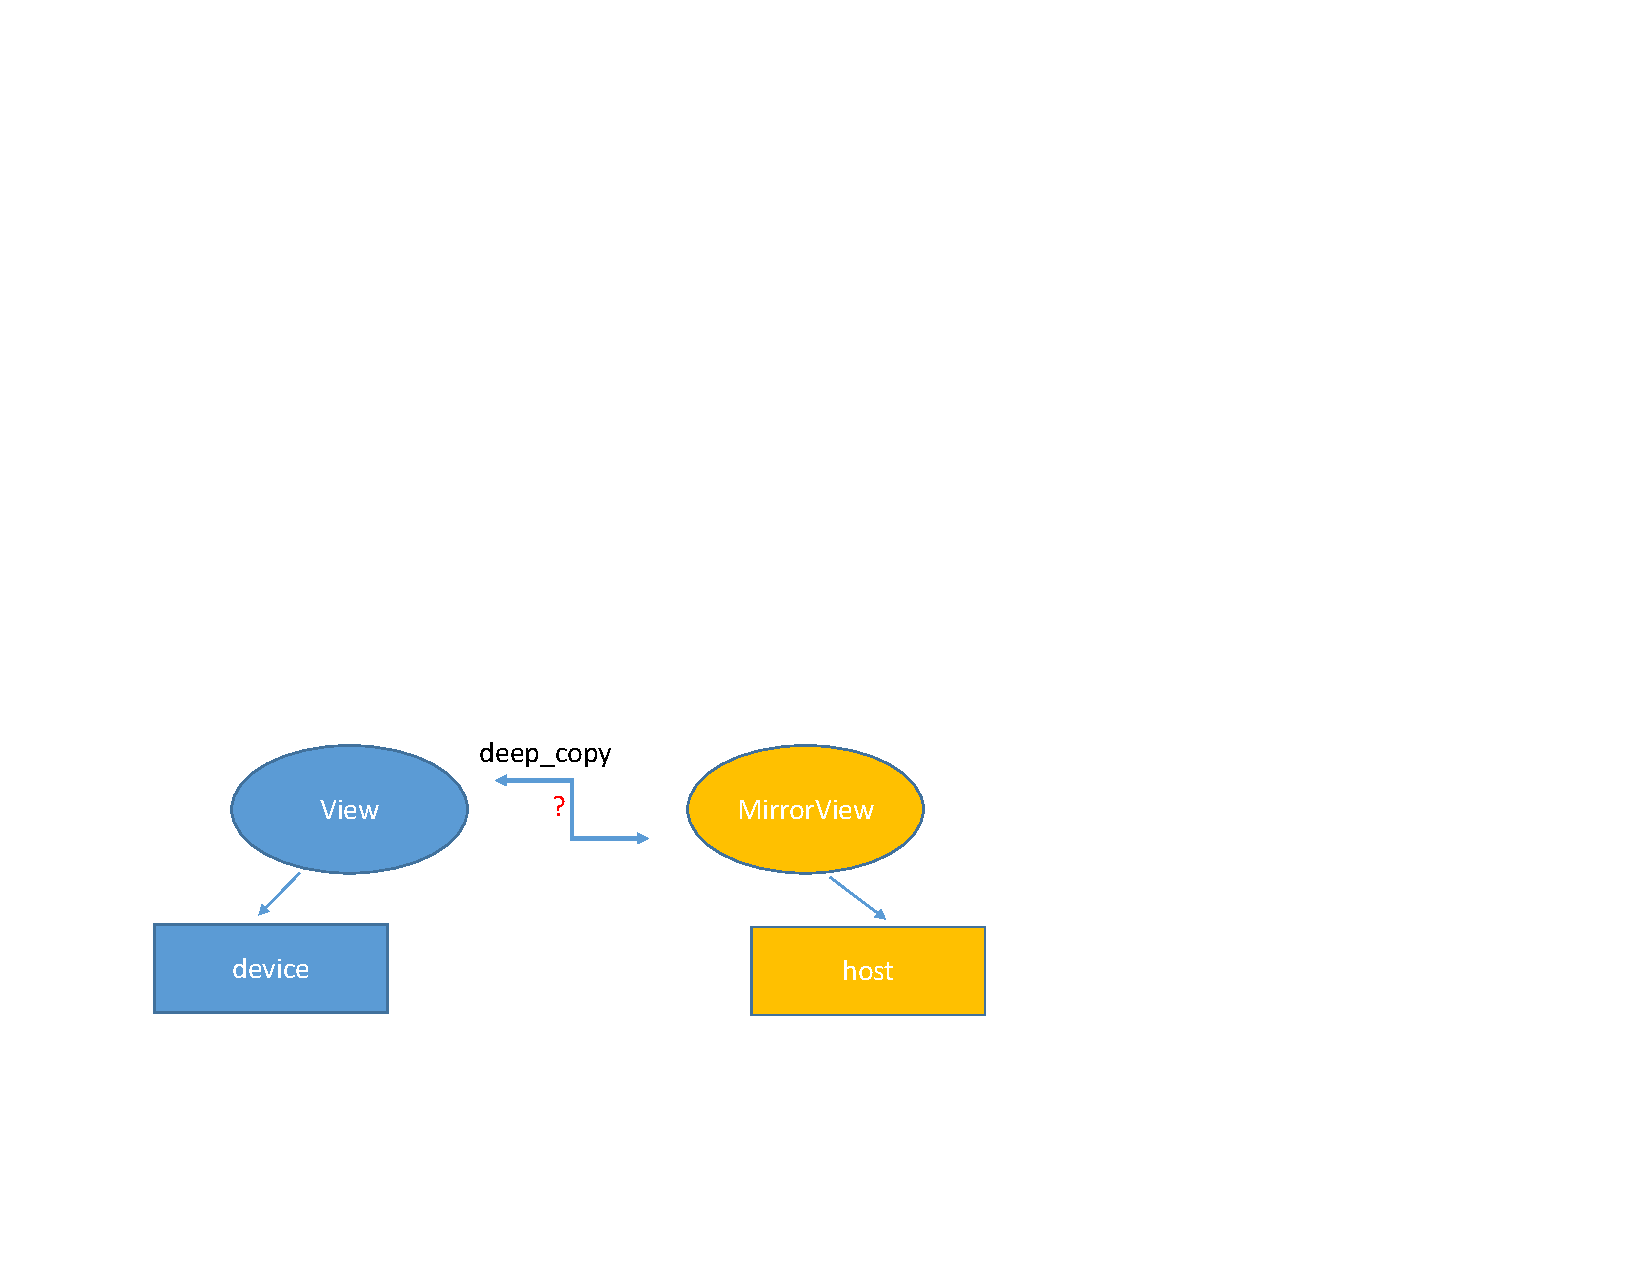
\includegraphics[height=1in]{figures/DualView_hostMirror.pdf}
\end{figure}

\textbf{Without DualView, could use MirrorViews, but}
  \begin{itemize}
    \item{deep copies are expensive, use sparingly}
    \item{do I need a deep copy here?}
    \item{where is the most recent data?}
    \item{is data on the host or device stale?}
    \item{was code modified upstream? is data here now stale, but not in previous version?}
  \end{itemize}

\end{frame}


%==========================================================================

\begin{frame}[fragile]{DualView: Usage}

\vspace{1em}
  \textbf{DualView bundles two views, a Host View and a Device View}

\begin{figure}[h]
 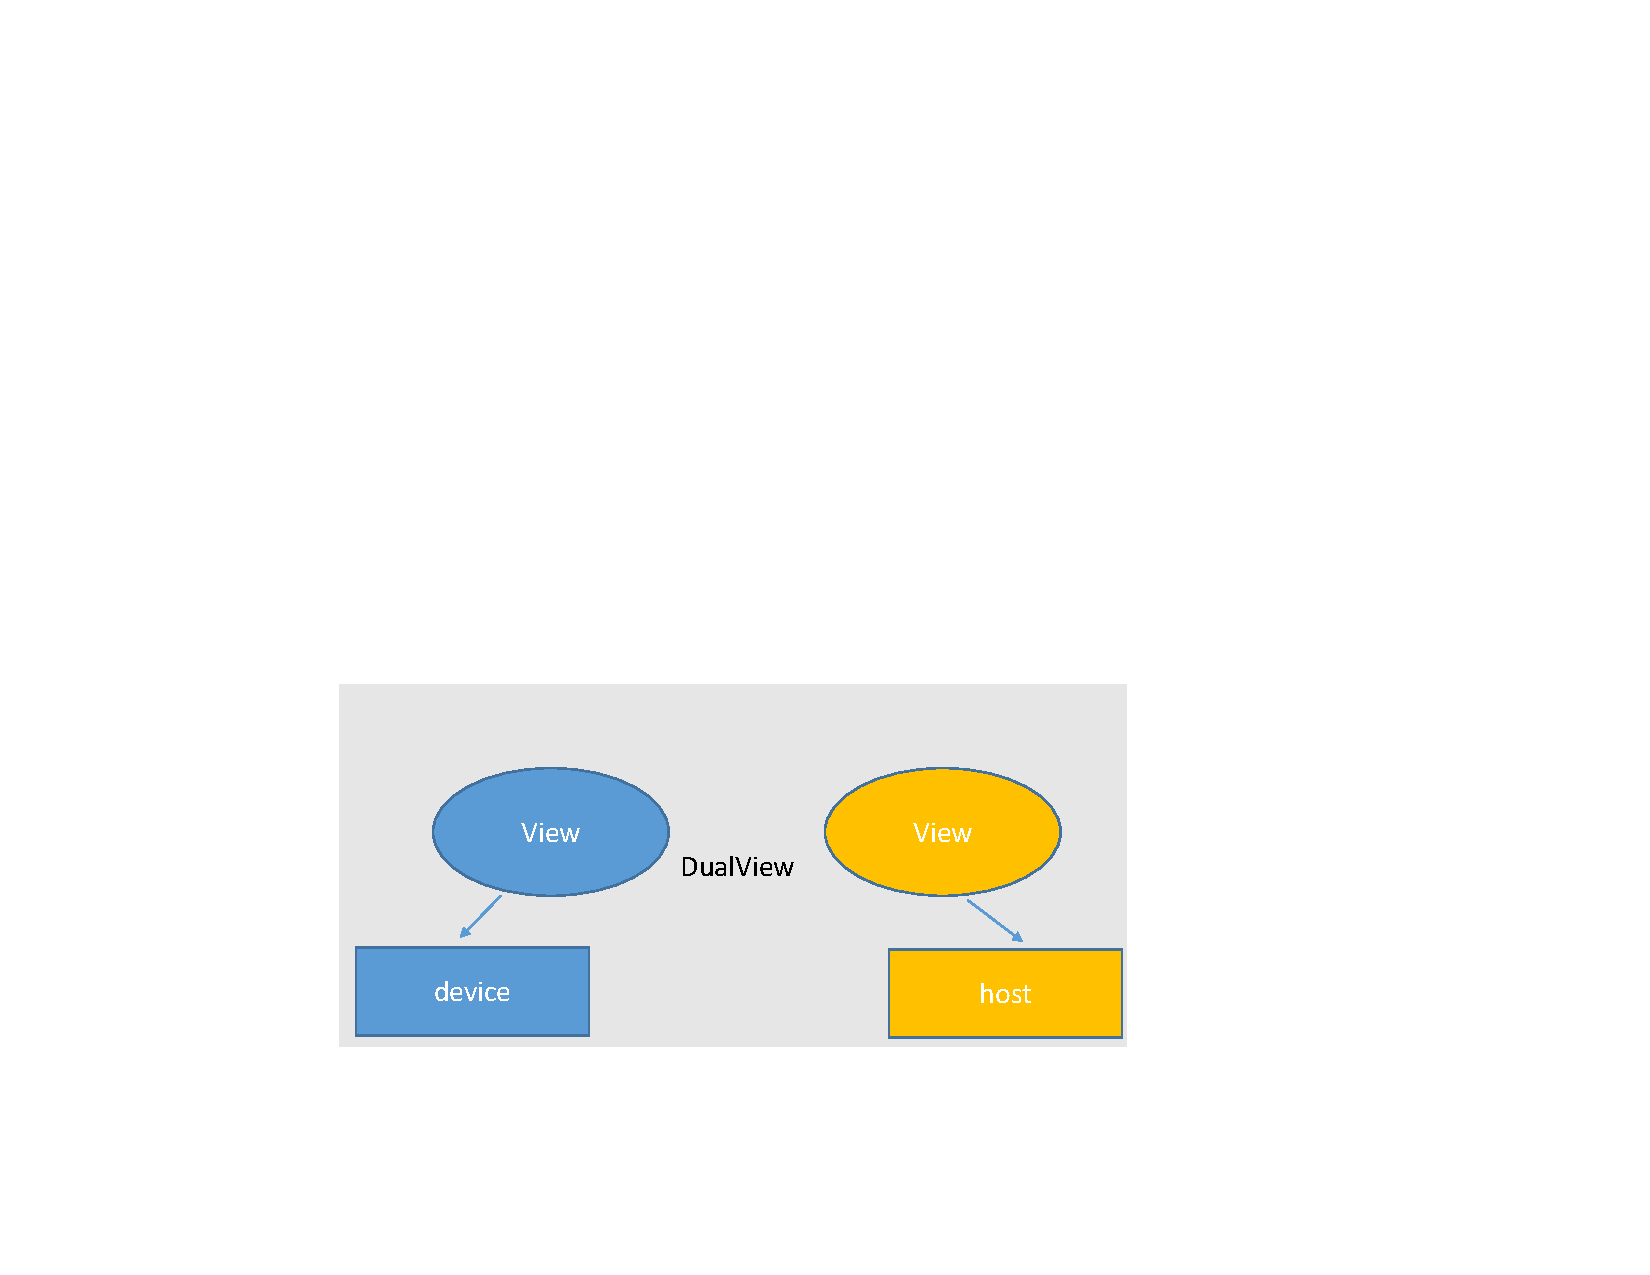
\includegraphics[height=1.25in]{figures/DualView_dualView.pdf}
\end{figure}

\textbf{There is no automatic tracking of data freshness:}
\begin{itemize}
\item  you must tell Kokkos when data has been modified on a memory space.
\item If you mark data as modified when you modify it, then Kokkos will know if it needs to move data
\end{itemize}
\end{frame}

%==========================================================================

\begin{frame}[fragile]{DualView: Usage(1)}
\vspace{1em}
  \textbf{DualView bundles two views, a Host View and a Device View}
  \begin{itemize}
    \item{Data members for the two views}
      \begin{code}[frame=single, keywords={}]
          DualView::t_host h_view
          DualView::t_dev  d_view
       \end{code}
    \item{Retrieve data members}
      \begin{code}[frame=single, keywords={}]
          t_host view_host();
          t_dev  view_device();
      \end{code}
    \item{Mark data as modified}
      \begin{code}[frame=single, keywords={}]
          void modify_host();
          void modify_device();
      \end{code}
  \end{itemize}
\end{frame}

\begin{frame}[fragile]{DualView: Usage(2)}
\vspace{1em}
  \textbf{DualView bundles two views, a Host View and a Device View}
  \begin{itemize}
    \item{Sync data in a direction if not in sync}
      \begin{code}[frame=single, keywords={}]
          void sync_host();
          void sync_device();
      \end{code}
    \item{Check sync status}
      \begin{code}[frame=single, keywords={}]
          bool need_sync_host();
          bool need_sync_device();
      \end{code}
   \end{itemize}
\end{frame}

\begin{frame}[fragile]{DualView: Usage in generic context}
\textbf{DualView has templated functions for generic use in templated code}

  \begin{itemize}
    \item{Retrieve data members}
      \begin{code}[frame=single, keywords={}]
          template<class Space>
          auto view();
      \end{code}
\vspace{-0.2em}
    \item{Mark data as modified}
      \begin{code}[frame=single, keywords={}]
          template<class Space>
          void modify();
      \end{code}
\vspace{-0.2em}
    \item{Sync data in a direction if not in sync}
      \begin{code}[frame=single, keywords={}]
          template<class Space>
          void sync();
      \end{code}
\vspace{-0.2em}
    \item{Check sync status}
      \begin{code}[frame=single, keywords={}]
          template<class Space>
          bool need_sync();
      \end{code}
   \end{itemize}   
\end{frame}

\begin{frame}[fragile]{DualView Example}

\begin{code}[keywords={sync_device,modify_device,view_device,view_host,sync_host,modify_host,DualView}]
class Foo {
DualView<...> data;
void run_a() {
  data.sync_device(); data.modify_device();
  auto d_data = data.view_device();
  parallel_for(N, KOKKOS_LAMBDA(int i) { d_data(i)+=/*mod d_d*/});
}
void run_b() {
  data.sync_host(); 
  auto h_data = data.view_host();
  for(int i=0; i<N; i++) { h_data(i) += /* modify h_data */ });
  data.modify_host();
}
void run_c() {
  data.sync_device();
  auto d_data = data.view_device();
  parallel_for(N, KOKKOS_LAMBDA(int i) { /* read d_data */ });
}
void do_operations(bool a, bool b, bool c) {
  if(a) run_a();
  if(b) run_b();
  if(c) run_c();
}
};
\end{code}
\end{frame}
%==========================================================================

\begin{frame}[fragile]{Exercise - DualView}

  \textbf{Details}:
  \begin{small}
  \begin{itemize}
    \item Location: \ExerciseDirectory{dualview/Begin}
    \item Modify or create a new compute\_enthalpy function in dual\_view\_exercise.cpp to:
    \begin{itemize}
      \item 1. Take (dual)views as arguments
      \item 2. Call \textbf{modify()} and/or \textbf{sync()} when appropriate for the dual views
      \item 3. Runs the kernel on host or device execution spaces
    \end{itemize}
  \end{itemize}
  \end{small}

\begin{code}
  # Compile for CPU
  cmake -B build_openmp -DKokkos_ENABLE_OPENMP=ON
  cmake --build build_openmp
  # Run on CPU
  ./build_openmp/dualview
  # Note the warnings, set appropriate environment variables
  # Compile for GPU
  cmake -B build_cuda -DKokkos_ENABLE_CUDA=ON
  cmake --build build_cuda
  # Run on GPU
  ./build_cuda/dualview
\end{code}

\end{frame}

%==========================================================================
